% Options for packages loaded elsewhere
\PassOptionsToPackage{unicode}{hyperref}
\PassOptionsToPackage{hyphens}{url}
\PassOptionsToPackage{dvipsnames,svgnames,x11names}{xcolor}
%
\documentclass[
  letterpaper,
  DIV=11,
  numbers=noendperiod]{scrartcl}

\usepackage{amsmath,amssymb}
\usepackage{iftex}
\ifPDFTeX
  \usepackage[T1]{fontenc}
  \usepackage[utf8]{inputenc}
  \usepackage{textcomp} % provide euro and other symbols
\else % if luatex or xetex
  \usepackage{unicode-math}
  \defaultfontfeatures{Scale=MatchLowercase}
  \defaultfontfeatures[\rmfamily]{Ligatures=TeX,Scale=1}
\fi
\usepackage{lmodern}
\ifPDFTeX\else  
    % xetex/luatex font selection
\fi
% Use upquote if available, for straight quotes in verbatim environments
\IfFileExists{upquote.sty}{\usepackage{upquote}}{}
\IfFileExists{microtype.sty}{% use microtype if available
  \usepackage[]{microtype}
  \UseMicrotypeSet[protrusion]{basicmath} % disable protrusion for tt fonts
}{}
\makeatletter
\@ifundefined{KOMAClassName}{% if non-KOMA class
  \IfFileExists{parskip.sty}{%
    \usepackage{parskip}
  }{% else
    \setlength{\parindent}{0pt}
    \setlength{\parskip}{6pt plus 2pt minus 1pt}}
}{% if KOMA class
  \KOMAoptions{parskip=half}}
\makeatother
\usepackage{xcolor}
\setlength{\emergencystretch}{3em} % prevent overfull lines
\setcounter{secnumdepth}{-\maxdimen} % remove section numbering
% Make \paragraph and \subparagraph free-standing
\ifx\paragraph\undefined\else
  \let\oldparagraph\paragraph
  \renewcommand{\paragraph}[1]{\oldparagraph{#1}\mbox{}}
\fi
\ifx\subparagraph\undefined\else
  \let\oldsubparagraph\subparagraph
  \renewcommand{\subparagraph}[1]{\oldsubparagraph{#1}\mbox{}}
\fi


\providecommand{\tightlist}{%
  \setlength{\itemsep}{0pt}\setlength{\parskip}{0pt}}\usepackage{longtable,booktabs,array}
\usepackage{calc} % for calculating minipage widths
% Correct order of tables after \paragraph or \subparagraph
\usepackage{etoolbox}
\makeatletter
\patchcmd\longtable{\par}{\if@noskipsec\mbox{}\fi\par}{}{}
\makeatother
% Allow footnotes in longtable head/foot
\IfFileExists{footnotehyper.sty}{\usepackage{footnotehyper}}{\usepackage{footnote}}
\makesavenoteenv{longtable}
\usepackage{graphicx}
\makeatletter
\def\maxwidth{\ifdim\Gin@nat@width>\linewidth\linewidth\else\Gin@nat@width\fi}
\def\maxheight{\ifdim\Gin@nat@height>\textheight\textheight\else\Gin@nat@height\fi}
\makeatother
% Scale images if necessary, so that they will not overflow the page
% margins by default, and it is still possible to overwrite the defaults
% using explicit options in \includegraphics[width, height, ...]{}
\setkeys{Gin}{width=\maxwidth,height=\maxheight,keepaspectratio}
% Set default figure placement to htbp
\makeatletter
\def\fps@figure{htbp}
\makeatother

\KOMAoption{captions}{tableheading}
\makeatletter
\makeatother
\makeatletter
\makeatother
\makeatletter
\@ifpackageloaded{caption}{}{\usepackage{caption}}
\AtBeginDocument{%
\ifdefined\contentsname
  \renewcommand*\contentsname{Table of contents}
\else
  \newcommand\contentsname{Table of contents}
\fi
\ifdefined\listfigurename
  \renewcommand*\listfigurename{List of Figures}
\else
  \newcommand\listfigurename{List of Figures}
\fi
\ifdefined\listtablename
  \renewcommand*\listtablename{List of Tables}
\else
  \newcommand\listtablename{List of Tables}
\fi
\ifdefined\figurename
  \renewcommand*\figurename{Figure}
\else
  \newcommand\figurename{Figure}
\fi
\ifdefined\tablename
  \renewcommand*\tablename{Table}
\else
  \newcommand\tablename{Table}
\fi
}
\@ifpackageloaded{float}{}{\usepackage{float}}
\floatstyle{ruled}
\@ifundefined{c@chapter}{\newfloat{codelisting}{h}{lop}}{\newfloat{codelisting}{h}{lop}[chapter]}
\floatname{codelisting}{Listing}
\newcommand*\listoflistings{\listof{codelisting}{List of Listings}}
\makeatother
\makeatletter
\@ifpackageloaded{caption}{}{\usepackage{caption}}
\@ifpackageloaded{subcaption}{}{\usepackage{subcaption}}
\makeatother
\makeatletter
\@ifpackageloaded{tcolorbox}{}{\usepackage[skins,breakable]{tcolorbox}}
\makeatother
\makeatletter
\@ifundefined{shadecolor}{\definecolor{shadecolor}{rgb}{.97, .97, .97}}
\makeatother
\makeatletter
\makeatother
\makeatletter
\makeatother
\ifLuaTeX
  \usepackage{selnolig}  % disable illegal ligatures
\fi
\IfFileExists{bookmark.sty}{\usepackage{bookmark}}{\usepackage{hyperref}}
\IfFileExists{xurl.sty}{\usepackage{xurl}}{} % add URL line breaks if available
\urlstyle{same} % disable monospaced font for URLs
\hypersetup{
  pdftitle={The Sinner},
  pdfauthor={Daniel Śliwiński},
  colorlinks=true,
  linkcolor={blue},
  filecolor={Maroon},
  citecolor={Blue},
  urlcolor={Blue},
  pdfcreator={LaTeX via pandoc}}

\title{The Sinner}
\author{Daniel Śliwiński}
\date{2023-06-10}

\begin{document}
\maketitle
\ifdefined\Shaded\renewenvironment{Shaded}{\begin{tcolorbox}[enhanced, boxrule=0pt, interior hidden, frame hidden, sharp corners, breakable, borderline west={3pt}{0pt}{shadecolor}]}{\end{tcolorbox}}\fi

\begin{center}\rule{0.5\linewidth}{0.5pt}\end{center}

\hypertarget{the-sinner}{%
\section{The Sinner}\label{the-sinner}}


\includegraphics{sinner_files/sinner.jpg}

\subsection{Brief Description of the TV Show}

\emph{``The Sinner''} is an American police procedural anthology
television series developed by \emph{``Derek Simonds''} for USA Network.
It is based on \emph{``Petra Hammesfahr's''} 1999 novel, which served as
the basis for the first season. The series stars \emph{``Bill Pullman''}
as a police detective who investigates crimes committed by unlikely
culprits and attempts to uncover their motivations. Only
\emph{``Pullman''} appears in every season, while the rest of the cast
mostly changes for each season's story.

The show was intended as an eight-part miniseries, but its success led
to it being turned into an anthology series, which aired for four
seasons from August 2, 2017, to December 1, 2021.

The first season of \emph{``The Sinner''} received nominations for the
\textbf{Golden Globe Award} for Best Miniseries or Television Film and
Best Actress -- Miniseries or Television Film for \emph{``Jessica
Biel''}. \emph{``Biel''} was also nominated for a \textbf{Primetime Emmy
Award} for Outstanding Lead Actress in a Limited Series or Movie.

The show captivates viewers with deep dive in to psyche of the main
characters, posing an essential question who are we and what is our dark
side?

\subsection{Critics Review}

\emph{Stuart Heritage}:

\begin{quote}
\mbox{}%
\hypertarget{what-is-it}{%
\paragraph{What is it:}\label{what-is-it}}

Let's call it a \emph{whydunnit}.
\end{quote}

\begin{quote}
\mbox{}%
\hypertarget{why-youll-love-it}{%
\paragraph{Why you'll love it:}\label{why-youll-love-it}}

A woman -- a normal, slightly dissatisfied woman -- goes to the beach.
She goes for a swim and, out of nowhere, is gripped by a strange
sensation. She returns to the shore, hugs her son, eats a pear and then
stabs a man to death.
\end{quote}

\begin{quote}
\textbf{Why?} Did she know the victim? Did his sexy seaside horseplay
bring back memories of some hidden trauma? Was it her medication? Her
bedroom wallpaper? Was it because -- as I initially suspected -- he was
playing music on his phone in a crowded area? The woman herself doesn't
seem to know. \emph{What's going on?} This is the central question at
the heart of \emph{The Sinner}.
\end{quote}

\begin{quote}
A sly ratings success in the US -- it has been the most-watched new
cable show this year -- \emph{The Sinner} is based on the Petra
Hammesfahr novel of the same name, and takes the form of a gussied-up
push and pull between the woman (played by Jessica Biel) and the
detective tasked with figuring out this mess (Bill Pullman).
\end{quote}

\begin{quote}
The problem with programmes that hinge on a gimmick as grabby as this is
that the answers are often much less satisfying than the inciting
incident. But the joy of \emph{The Sinner} is getting to watch Biel do
everything in her power to just get the ordeal over with. A more
traditional show would turn the relationship between her and Pullman
into a cat and mouse, but that isn't really the case here. The mouse is
splayed out on the floor begging to be eaten and the cat can't
understand why.
\end{quote}

\begin{quote}
She instantly pleads guilty to avoid a trial. But a competency
evaluation is ordered, so she explains her motivation in horrific
detail. But that's quickly revealed to be a lie, so the process must
begin anew. Biel would rather spend her life rotting in prison than
truly examine her actions, but every detail that floats to the surface
-- drug problems, a cartoonishly awful childhood, sexy flashbacks of
undulating bodies -- starts to make that impossible. Before you know it,
these flashbacks have piled up on top of more flashbacks and the whole
thing edges towards the precipice. It gets to the point where the
faintest prod could derail the entire series, so the fact that it
doesn't is nothing short of a miracle.
\end{quote}

\begin{quote}
Fortunately, there are answers. This is no \emph{Lost}-style
wheel-spinning exercise, and the denouement is just as satisfying and
horrible as the conclusion to the first \emph{Broadchurch}. If you find
yourself drifting away during \emph{The Sinner's} midpoint, I can
promise you it's worth persevering with.
\end{quote}

\begin{quote}
As bracingly vanity-free as Biel's performance is, all blood and gut and
scab, Pullman is the real secret weapon here. His detective is rumpled
and kinky, like Columbo if old Columbo episodes were routinely
interrupted by scenes of him getting pegged by a dominatrix. He's
horribly, horribly sad, and you sense that he has only seized upon this
case because it's the one part of his life that he can control. Not to
give anything away, but the show ends on such a note of finality that
the only way forward would be to shove Pullman into a new mystery next
year. Based on this run, that would be no bad thing.
\end{quote}

\href{https://www.theguardian.com/tv-and-radio/2017/nov/09/the-sinner-review-the-psychological-whydunnit-thats-been-a-big-us-ratings-success}{Source}

\begin{center}\rule{0.5\linewidth}{0.5pt}\end{center}

\hypertarget{the-sinner-a-statistical-overview}{%
\section{The Sinner: A Statistical
Overview}\label{the-sinner-a-statistical-overview}}

\paragraph{Viewership Analysis}

The \emph{The Sinner} has had a dynamic viewership over its four
seasons. The first season was met with a great reception, averaging
\textbf{1.8 million} viewers per episode. This success led to the
transformation of the show from an intended mini-series to a
full-fledged multi-season series.

However, subsequent seasons saw a decline in viewership. The numbers
fell to an average of \textbf{1.13 million} viewers per episode in the
second season. The trend continued with the third season, which drew in
an average of \textbf{0.65 million} viewers, and the fourth season,
attracting an average of \textbf{0.45 million} viewers per episode.

While I found each season's story incredibly captivating, it seems that
not everyone shares my feelings towards the later seasons.

\paragraph{Rotten Tomato ratings for each season:}

\begin{longtable}[]{@{}lll@{}}
\caption{Rotten Tomato Ratings for Each Season}\tabularnewline
\toprule\noalign{}
Season & Tomatometer & Audience\_Score \\
\midrule\noalign{}
\endfirsthead
\toprule\noalign{}
Season & Tomatometer & Audience\_Score \\
\midrule\noalign{}
\endhead
\bottomrule\noalign{}
\endlastfoot
Season 1 & 91\% & 87\% \\
Season 2 & 97\% & 82\% \\
Season 3 & 85\% & 46\% \\
Season 4 & 88\% & 77\% \\
\end{longtable}

As the table shows, season 3 performed the worst, according to the
audience score. However, critics rated season 2 slightly higher than the
first season, as per the Tomatometer score.

\paragraph{Average viewership over the four seasons}

\begin{figure}

{\centering 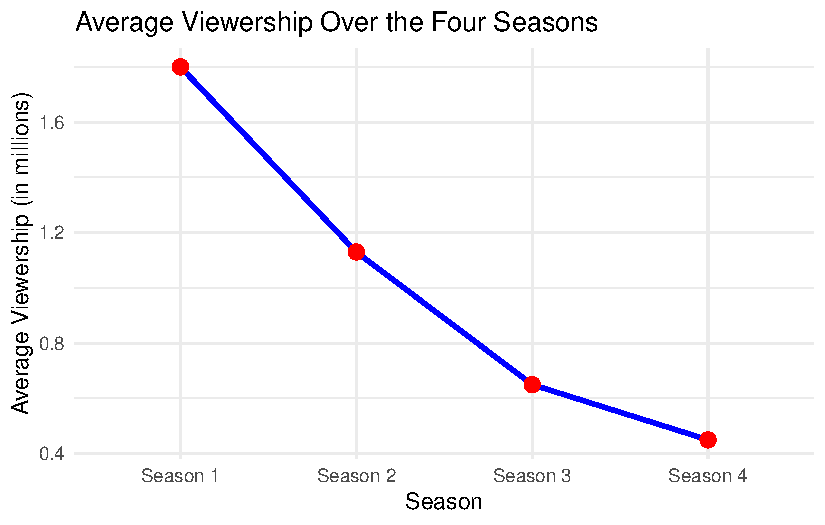
\includegraphics{sinner_files/figure-pdf/unnamed-chunk-2-1.pdf}

}

\caption{Average viewership over the four seasons}

\end{figure}

\paragraph{Change in viewership from season to season}

\begin{figure}

{\centering 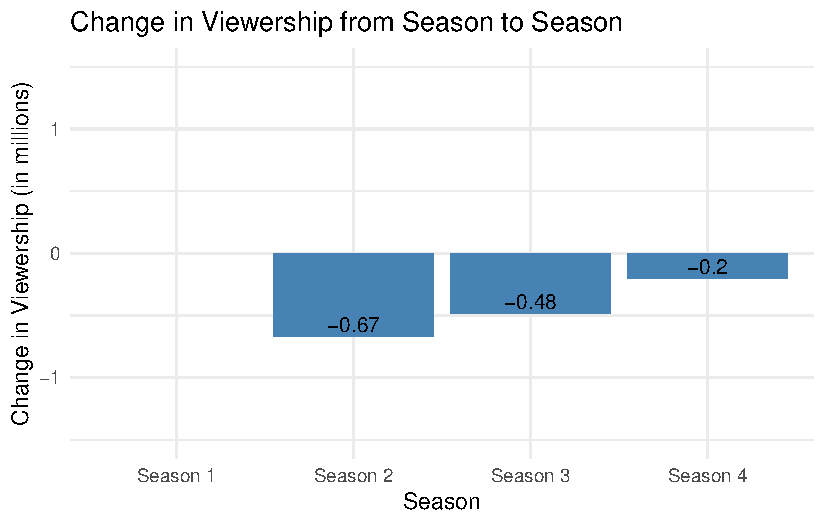
\includegraphics{sinner_files/figure-pdf/unnamed-chunk-3-1.pdf}

}

\caption{Change in viewership from season to season}

\end{figure}

Between the first and the second season, the viewership decreased by
-0.67 million. The trend continued in the subsequent seasons, with a
drop of -0.48 million viewers between the second and the third season,
and -0.2 million viewers between the third and the fourth season. This
consistent decrease in viewership may reflect various factors, such as
changes in the series' direction, competition with other shows, or
shifts in audience preferences.



\end{document}
